\chapter{Related Work} \label{chap:sota}

\section{Introduction}

 The following chapters introduces the two main topics dealt with in this dissertation (merge conflicts and the usage of large language models for software verification and test generation). They explore related work and how we can build on it to develop our approach.

\section{Semantic Conflict Detection}

The study of merge techniques and conflicts has a long history, likely even predating the specific terminology itself. Thus there is a large corpus of work to explore

Several related works exist which seeks to develop methods that can more systemically identify adulterated behaviour arising from semantic conflicts.

\subsection{Automated Behaviour Change Detection}

By Da Silva et al, we find an attempt at identifying cases of semantic conflict by applying automated behaviour change detection~\citep{kn:leuson}. In summary, with a base commit B, a left L, right R and merge M, they observe that a generated unit test that passes in L but fails in B partially reveals the effect of the changes made in that branch. If the test then fails in M, it is likely the changes made in R interfere. To generate unit tests they used EvoSuite and Randoop~\citep{kn:randoop}
~\citep{kn:evosuite}.

In their analysis they found that the developed tool only detected interference in four out of 15 changes within merge scenarios that do actually suffer from interference, corresponding then to a recall of 0.267. While this is a very modest rate, it displayed no false positives (precision of 1) and thus could likely be integrated in a testing process to prune possible merge conflicts early, or further studied and refined.



\subsection{Unit Tests}

In identifying the presence of semantic conflicts in a merge conflict, developed solutions have focused on the automatic generation of unit tests. Building upon their previous work, Da Silva et al ~\citep{kn:leuson2} worked with this approach: by proposing SAM (SemAntic Merge), a tool that generates tests upon merges in Java. In summary, SAM initially does a simple textual merge to integrate the difference branches while identifying possible textual conflicts. After merging four program versions are built, to fully describe the merge scenario under test: Base, Left, Right, Merge. Source code transformations to improve testability are also part of the process, but optional. Finally, the test generation tools are fed objects serialized during the execution of existing test suites. After applying four test generations tools: Evosuite ~\citep{kn:evosuite}, Differential Evosuite, Randoop ~\citep{kn:randoop} and Randoop Clean, their own adapted version of Randoop, SAM executes the generated tests against the four versions of the program, identifies which tests failed, interpreting it with pre-defined interference criteria heuristics and from there reports conflicts, if detected ~\citep{kn:leuson2}.

With detections in 9 out of 28, it shows improvements over previous work: the authors specifically highlight the best performance when combining tests from only EvoSuite and Differential EvoSuite. In both cases, they highlight the ability of transformations (for example, making private fields public) to increase testability, showing moderate improvements in some tested scenarios: "We observe that the adoption of Testability Transformations help the tools
to detect behavior changes. In the same direction as for semantic conflict
detection, 20 additional changes are detected with testability executables,
when compared to the original executables (only 69 changes detected). From
the 19 false-negative cases observed in the experiment, we could detect
behavior changes in 11 of them. However, the reported behavior changes are
not caused by the changes involved in the semantic conflicts. So we can’t say
that the tools were close in these cases."  ~\citep{kn:leuson2}.


Nuno Castanho has proposed the tool UNSETTLE (aUtomatic uNit teSt gEneraTion for semanTic confLict dEtection) ~\citep{kn:nuno}. This tool is composed of two modules:

Changes-Matcher identifies the possible presence of semantic conflicts, by first computing the changes between different versions (base and variants) and then comparing it to a set of patterns describing common sources of conflicts as a base. From this it generates a DSL file, highlighting which methods and classes should be put under test to identify the conflict.

The second module is the test generator, a modified version of EvoSuite that takes the previously created artifact as an input to guide test generation.

Of particular interest to us is Changes-Matcher, as this is also the starting point for our work, with the usage of a LLM over EvoSuite for test generation instead.

\subsection{Regression Testing}

Ti Jao et al have proposed test oracles for program merges. Most significantly, not only do they support two and three way merges but also octopus merges. The developed tool, TOM, generates tests to identify unexpected and lost behaviour. \citep{kn:ji2022}

\section{Test Generation}

\subsection{Traditional Automatic Test Generation}

Traditional methods of automated test generation can be divided into random and search-based techniques. The former, being random, is simpler and faster, while the latter employs heuristics and search algorithms to fulfill some criteria, like maximizing code coverage.

Randoop is one such example of random test generation. Some of the disadvantages of this technique can be mitigated with the employment of feedback-direction. ~\citep{kn:randoop} Effectively, the search space of possible random tests is pruned, by guiding the test generator towards valid cases, avoiding expansion on invalid test cases~\citep{kn:randoop}.

Evosuite implements search-based automatic test generation for Java code, aiming for tests that achieve high coverage, while being as small as possible and providing assertions. To achieve this they implement both evolutionary search to evolve the suite with respect to a coverage criterion and mutation testing to generate assertions~\citep{kn:evosuite}.

EvosuiteR extends Evosuite, aiming to provide automated generation of regression tests. Thus it takes account two versions of the software and aside from coverage, it considers state distance ("how different is the state of
all objects in the test suite across the two versions") and control flow distance ("how
far are the two versions from diverging")~\citep{kn:evosuiter}.


Similar suites have been developed, for example, for Python ~\citep{kn:pynguin}.

\subsection{Test Generation with LLM's}

The recent explosion in complexity and popularity of LLM's has suscitated developer interest in their abilities with regards to accelerate and automate software engineering. Angela Fan et al identified that by 2023 3\% of pre-prints were related to Large Language Models and 11\% of those related to their use in software engineering.\cite{kn:angela} Particularly relevant is their ability to generate tests, with an expectation that they could achieve better coverage, correctness and readability than previous techniques of automated test generation.\cite{kn:junjiewang}
In comparison to traditional suites for automated test generation, such as EvoSuite, Palus, Randoop, and JTExpert, ChatGPT has shown, given right tuning of temperature settings, to evidentiate equivalent robustness\cite{kn:gptunitbra}.
From surveys done on the topic, we find Codex and GPT variants to be the most commonly used LLM's for this issue. \cite{kn:junjiewang}

While many studies suggest LLM's are competitive with traditional methods of software generation, we can also find evidence to the contrary. Specifically, testing across several LLM's, including Codex, StarCoder and GPT-3.5-Turbo, shows they fail in all regards compared to Evosuite, primarily due to the generation of non-compilable code, often due to "hallucination" of non-existent types and methods. \citep{kn:siddiq2023empirical}. Yutian Tang and others find Evosuite outperforms ChatGPT in code coverage. \citep{kn:tang2023chatgpt}. Given the novelty of the technology, it is unsurprising there is such variance in reported results and research, but it is worth investigating.

Despite variable conclusions regarding correctness and coverage, it seems generally agreed that ChatGPT is good at generating readable code. Yutian Tang et al highlight that despite minor style errors, primarily in identation, the generated code is clear and easy to understand. \citep{kn:tang2023chatgpt}. A survey of software developers has found ChatGPT to have comparable and even better readability than manually written tests. \citep{kn:chattester}


Given the LLM can produce unreliable results, the maximization of ChatGPT's abilities with regards to test generation has been explored: techniques such as prompting the LLM for a explanation of what the code is intending to do \cite{kn:nuances} and feeding error messages from codes that fail to compile or execute as intended back to the LLM for correction \cite{kn:chattester} have shown an amazing capacity for test generation, given the right prompting.

Regarding prompting, understanding how to best engineer prompts to achieve the desired output from the LLM is a particularly relevant issue. For example, in the generation of test inputs, research found “generate diverse test input” to be preferable over “generate test inputs that result in different outputs between PUT and reference versions”, as ChatGPT could not accurately identify the nuances required to correctly carry out the latter's instructions. \citep{kn:nuances}
With unit testing generation in particular, Zhiqiang Yuan et al, in developing the ChatTester tool, highlight the importance of combining a natural language descriptor with the appropriate code context. \citep{kn:chattester}
\begin{figure}[!h]
    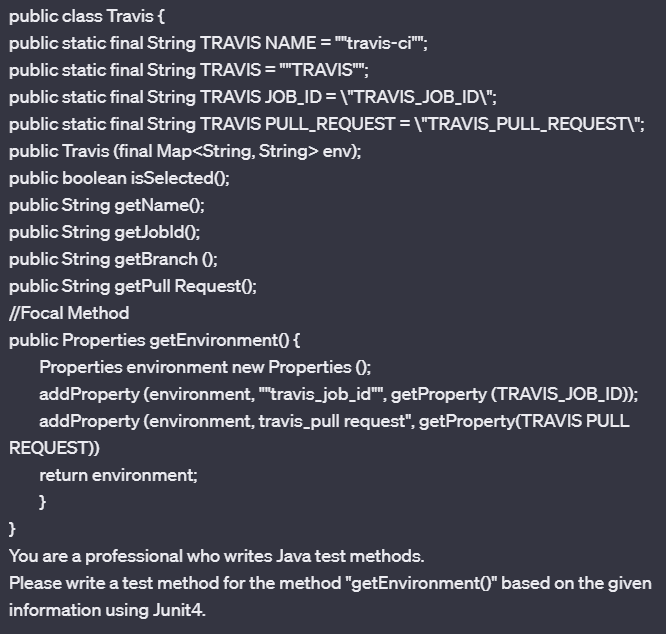
\includegraphics[width=0.86\textwidth]{figures/basicprompt.jpg}
    \caption{Basic Prompt in ChatTester}
    \label{fig:arch}
\end{figure}
\begin{figure}[!h]
    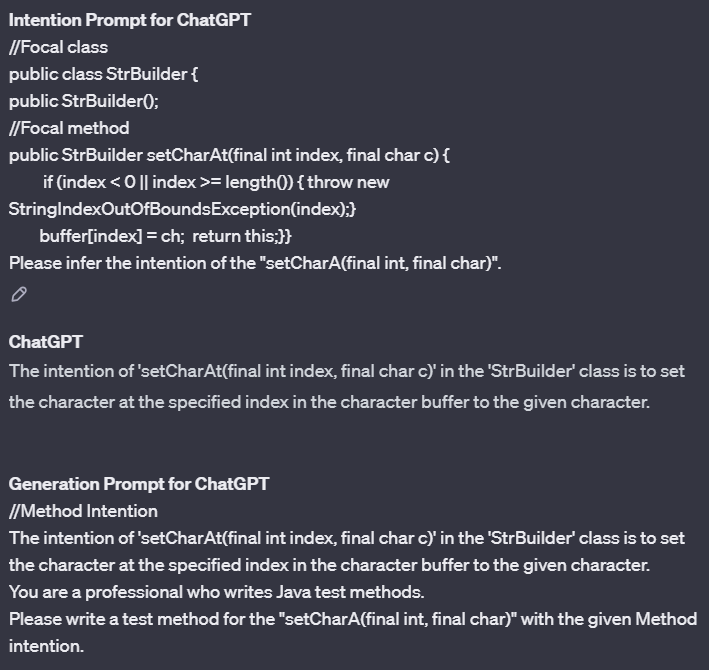
\includegraphics[width=0.86\textwidth]{figures/inferenceprompt.jpg}
    \caption{Inference Prompt in ChatTester}
    \label{fig:arch}
\end{figure}

While they argue that it is little known how effective these strategies are, J.D. Zamfirescu-Pereira and others highlight several prompting strategies: give examples of desired interaction, write prompts that look somewhat like code and repeat yourself \citep{kn:johnny}. They note difficulties participants have in prompt generation, such as avoiding giving examples due to fear the LLM will simply replicate it, difficulty in searching online for help and adapting existing solutions and overgeneralizing from a single example \citep{kn:johnny}.

In prompting we can distinguish a few types of prompts: zero-shot, where instructions are simply given, few-shot, where examples of inputs and outputs are given and few-shot with preamble, combining the previous two examples to give both a preamble instructing the LLM on what to achieve, follow by examples of inputs and outputs \citep{kn:promptprofiannaca}

Given the natural language aspect of LLM prompting is one the features that most distinguishes it from classical programming, it is worth exploring methods of systematizing it, making it work more like code. It is with this objective that LMQL (Language Model Query Language) was developed, introducing a scripting based query language \citep{kn:lmql}. Evidence shows it reduces computing costs by up to 80\% \citep{kn:lmql}.

The team behind ChatUniTest presents a two step prompting system, where instructions of what is to be done and how are first provided: "Please help me generate a JUnit test for a specific Java method using JUnit5 and Mockito3. I will provide the source code for the method, relevant method signatures and fields, required dependencies, Java class containing the method, expected behavior, and involved classes in the project. Create a test that imports necessary dependencies, compiles without errors, and achieves maximum branch and line coverage. No explanations needed.". This is followed by a prompt with the information proper for the creation of the test: "The focal method is ... in the class ... , and the class information is .... The brief information of involved class ... is ..." \citep{kn:chatunitest}


The training of LLM's in open source repositories gives cause to the fear that automatic test generation might be reliant on the model being trained in the code under test, or simply replicating existing testing suites. To assuage this, it was identified that even when generating tests for packages hosted in GitLab (which were not used to train the LLM under study, gpt3.5-turbo), they still maintained high coverage. In addition, it was found that 60.0\% of the tests had <= 40\% similarity to existing tests and 92.8\% had <= 50\%. Thus we can conclude the LLM is not simply copying tests from the training set without alteration.\citep{kn:max}.


\section{Conclusions}


The related work aids our own work in several ways: the work explored as regards unit test generation can provide show us a baseline functioning of the idea we're trying to implement. Particularly, we can use their statistics regarding percentage of conflicts found to assess whether our own solution is an improvement with regards to previous work.

Crucially important too is the work of Nuno Castanho and, as previously mentioned, the developed Changes-Matcher ~\citep{kn:nuno}.

The study of works on LLM test generation should also prove useful in the future, allowing us to get a better understanding of their functioning and capabilites, as well as providing ideas and prompt generation techniques which we may have to apply in the future.